
\documentclass[12pt,a4paper]{article}
\usepackage{graphicx}
\begin{document}

\title{ Text alignment knowledge requirement analysis}
\author{Bartosz Kalińczuk}
\date{\today}
\maketitle

\newpage
\begin{abstract}
The purpose of this final master degree project was to experiment with various algorithms for speech and text alignment either with granularity of sentences, single words or even single phonemes. The output of this study was expected to find out how little data is necessary to compute a proper alignment. This project focuses mainly on Polish language, however it can be quite easily generalized for different languages. It also focuses solely on a audio with quite low level of noise, since  it introduces a lot of problems, and is out of the scope of this project.
\end{abstract}


\newpage
\tableofcontents

\newpage
\section{Introduction}

\newpage
\begin{center}
    \section{Speech signal}
\end {center}
\subsection{Human factor}

Speech is a most efficient way the human communicate. For generations this process was refined by evolution, so we can easily exchange messages even in hard situations. For this purpose our vocal mechanisms must well cooperate with our hearing ability. There is a certain set of sounds we can produce and our ears evolved to hear them as well as possible.\newline 

What is sound? According to dictionary: „Vibrations transmitted through an elastic solid or liquid or gas, with frequencies in the approximate range of 20 to 20000 hertz, capable of being detected by human organs of hearing”. [1]\newline

How do we hear? Human ear consist about 30000 hair-cells, which can convert mechanical wave of the sound into electromagnetic wave inside auditory nerves [2]. 
Each of these cell is excited by different frequency of mechanical wave of internal ear fluids, so it is no surprise, that people can hear only a certain range of frequencies, as stated in definition. These we expect to be finely tuned to the range of the sounds we can produce. Although it seems, that we can hear a bit more, but as we don't need that, it happens, that as we grow older, our hearing range is getting smaller, because our hear cells fail sometimes, but mostly those responsible for high frequencies, which we don't use too often.\newline

Humans can hear frequencies, that begins as low as 12Hz (under laboratory conditions) to 20kHz (for adults usually much lower). However speech range is a little bit smaller than that [3]: \newline

\begin{center}
    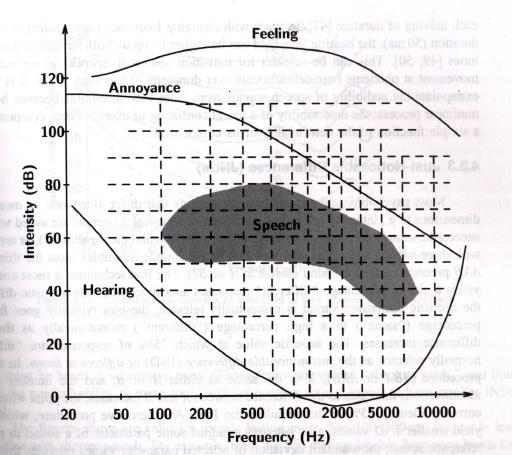
\includegraphics[scale=0.38]{speech_range.jpg}
\end {center}


\newpage
\subsection{Mel scale}

How we perceive sound, that is completely different matter and topic for long philosophical discussion. However we can help ourselves with some subjective experiments. For example Stevens, Volkman and Newman conducted an experiment on a number of listeners to measure, what do we perceive as equally distanced pitches. In this experiment, the participants of the experiment were asked to judge if given pitches were in equal distances. The output was, that humans don't experience sound linearly respectively to the frequency scale, but a perceptual scale was closer to logarithmic one. [5] \newline

Certain formulas were conceived to translate frequency scale to one, that is closer to how human actually perceive sound. \newline

One popular is mel scale, where mel comes from melody: [6] \newline
\begin{equation}
    m = 2595log_{10}(1 + \frac{f}{700})
\end{equation}
	
What looks like that:
\begin{center}
    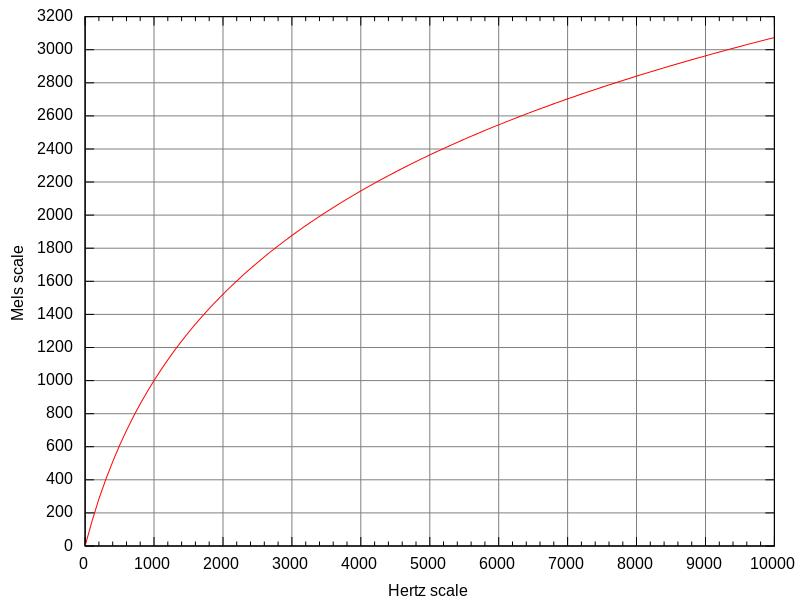
\includegraphics[scale=0.3]{mel_scale.jpg}
\end {center}

Another popular formula of so called bark scale, which is based on perception of loudness of the sound and proposed by Eberhard Zwicker in 1961. [7] \newline
\begin{equation}
    Bark = 13 atan(\frac{0.76f}{1000}) + 3.5 atan(\frac{f^2}{7500^2})
\end{equation}
In this project we use mel scale implemented in sphinx library, although bark scale is becoming more popular recently.

\newpage
\subsection{Frequency spectrum}

The conclusion from the anatomy of human ear is, that frequencies of the sound are important.
How can we obtain frequency spectrum from a digitized sound, so we can proceed further? \newline
The obvious tool for conversion of discrete function to frequencies is Discrete Fourier Transform, named after Jean Baptiste Joseph Fourier it is one of the most often used techniques of modern times. \newline

It all started from the postulate, that a heat equation can be satisfied by function of form: [11] \newline
\begin{equation}
    f(x)=\sum_{n=0}^N(A_n cos(nx) + B_n sin(nx))
\end{equation}
or in complex form:
\begin{equation}
    f(\theta)=\sum_{n=-\infty}^{\infty} C_n e^{i n \theta}
\end{equation}

Basically we convert our function's domain to frequency domain or to domain of sinusoidal functions. $C_n$ coefficients are complex values that encode both amplitude and phase of the converted signal/function at each frequency. \newline

The coefficients for any integrable functions over an interval $[\frac{-T}{2}, \frac{T}{2}]$ can be obtain using formula: [11] \newline
\begin{equation}
    C_n=\int_{\frac{-T}{2}}^{\frac{T}{2}} f(x) e^{-2 \pi i \frac{n}{T} x} dx
\end{equation}

or for the discrete case:
\begin{equation}
    C_k=\sum_{n=0}^{N-1} x_n e^{\frac{-2 \pi i k n}{N}} dx
\end{equation}
	

So far we haven't found any use in the speech recognition for phase part of the coefficients, however amplitude determines how powerful is signal at given frequency. The power value is given by:
\begin{equation}
    |X_k|/N = \sqrt{\Re(X_k)^2 + \Im(X_k)^2} / N
\end{equation}

\newpage
A sample conversion:
\begin{center}
    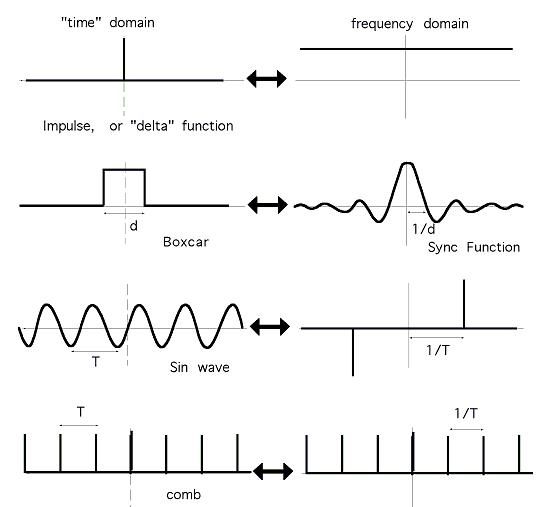
\includegraphics[scale=0.3]{sample_dft_conversion.jpg}
\end {center}

What size of the window should we use? First we have to notice, that in order to capture certain frequency, the window needs to be large enough. We would like to examine signals of frequency ranged from 100Hz (see speech frequencies ranges in chapter 2.1), which is a period of 100th of the second, so a 10millisecond window would be our bottom limit. \newline

Also windows with abrupt signal discontinuities may cause result with spectral artefacts, so a windowing function is usually applied. Popular choice is a Hamming window function: [8]
\begin{equation}
   w_j = 0.54 - 0.46 cos(\frac{2 \pi j}{W - 1}) 
\end{equation}
Which's plot is:
\begin{center}
    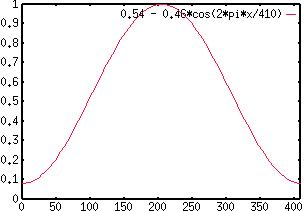
\includegraphics[scale=0.3]{hamming_window.jpg}
\end {center}

Note that it emphasises values in the middle of the window, so our actual windows should overlap to cover whole time domain. For example by shifting a window by a percentage of it actual width:
\begin{center}
    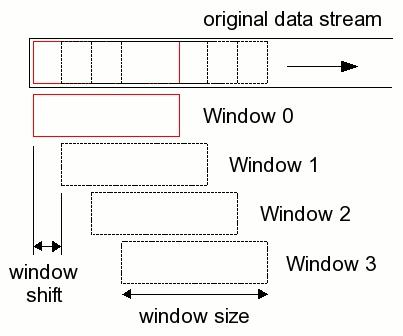
\includegraphics[scale=0.3]{window_shifting.jpg}
\end {center}


\end{document}
